\documentclass[border=10pt]{standalone}
\usepackage{tikz}
\usetikzlibrary{arrows.meta, positioning, shadows, calc}

\definecolor{boxblue}{HTML}{e8f4f8}
\definecolor{boxborder}{HTML}{2c3e50}
\definecolor{boxgrey}{HTML}{f0f0f0}
\definecolor{bordergrey}{HTML}{999999}
\definecolor{divider}{HTML}{aaaaaa}

\tikzset{
    model/.style={
        rectangle, rounded corners=4pt,
        draw=boxborder, fill=boxblue,
        minimum width=3.2cm, minimum height=1.1cm,
        text width=3.0cm, align=center,
        font=\small, drop shadow={shadow xshift=0.5mm, shadow yshift=-0.5mm}
    },
    unselected/.style={
        rectangle, rounded corners=4pt,
        draw=boxborder, fill=boxgrey,
        minimum width=3.2cm, minimum height=1.1cm,
        text width=3.0cm, align=center,
        font=\small, drop shadow={shadow xshift=0.5mm, shadow yshift=-0.5mm}
    },
    row label/.style={
        font=\scriptsize\itshape, text=bordergrey,
        align=right, text width=2.2cm
    },
    arr/.style={-Stealth, thick, color=boxborder},
    arr branch/.style={-Stealth, thin, color=boxborder}
}

\begin{document}
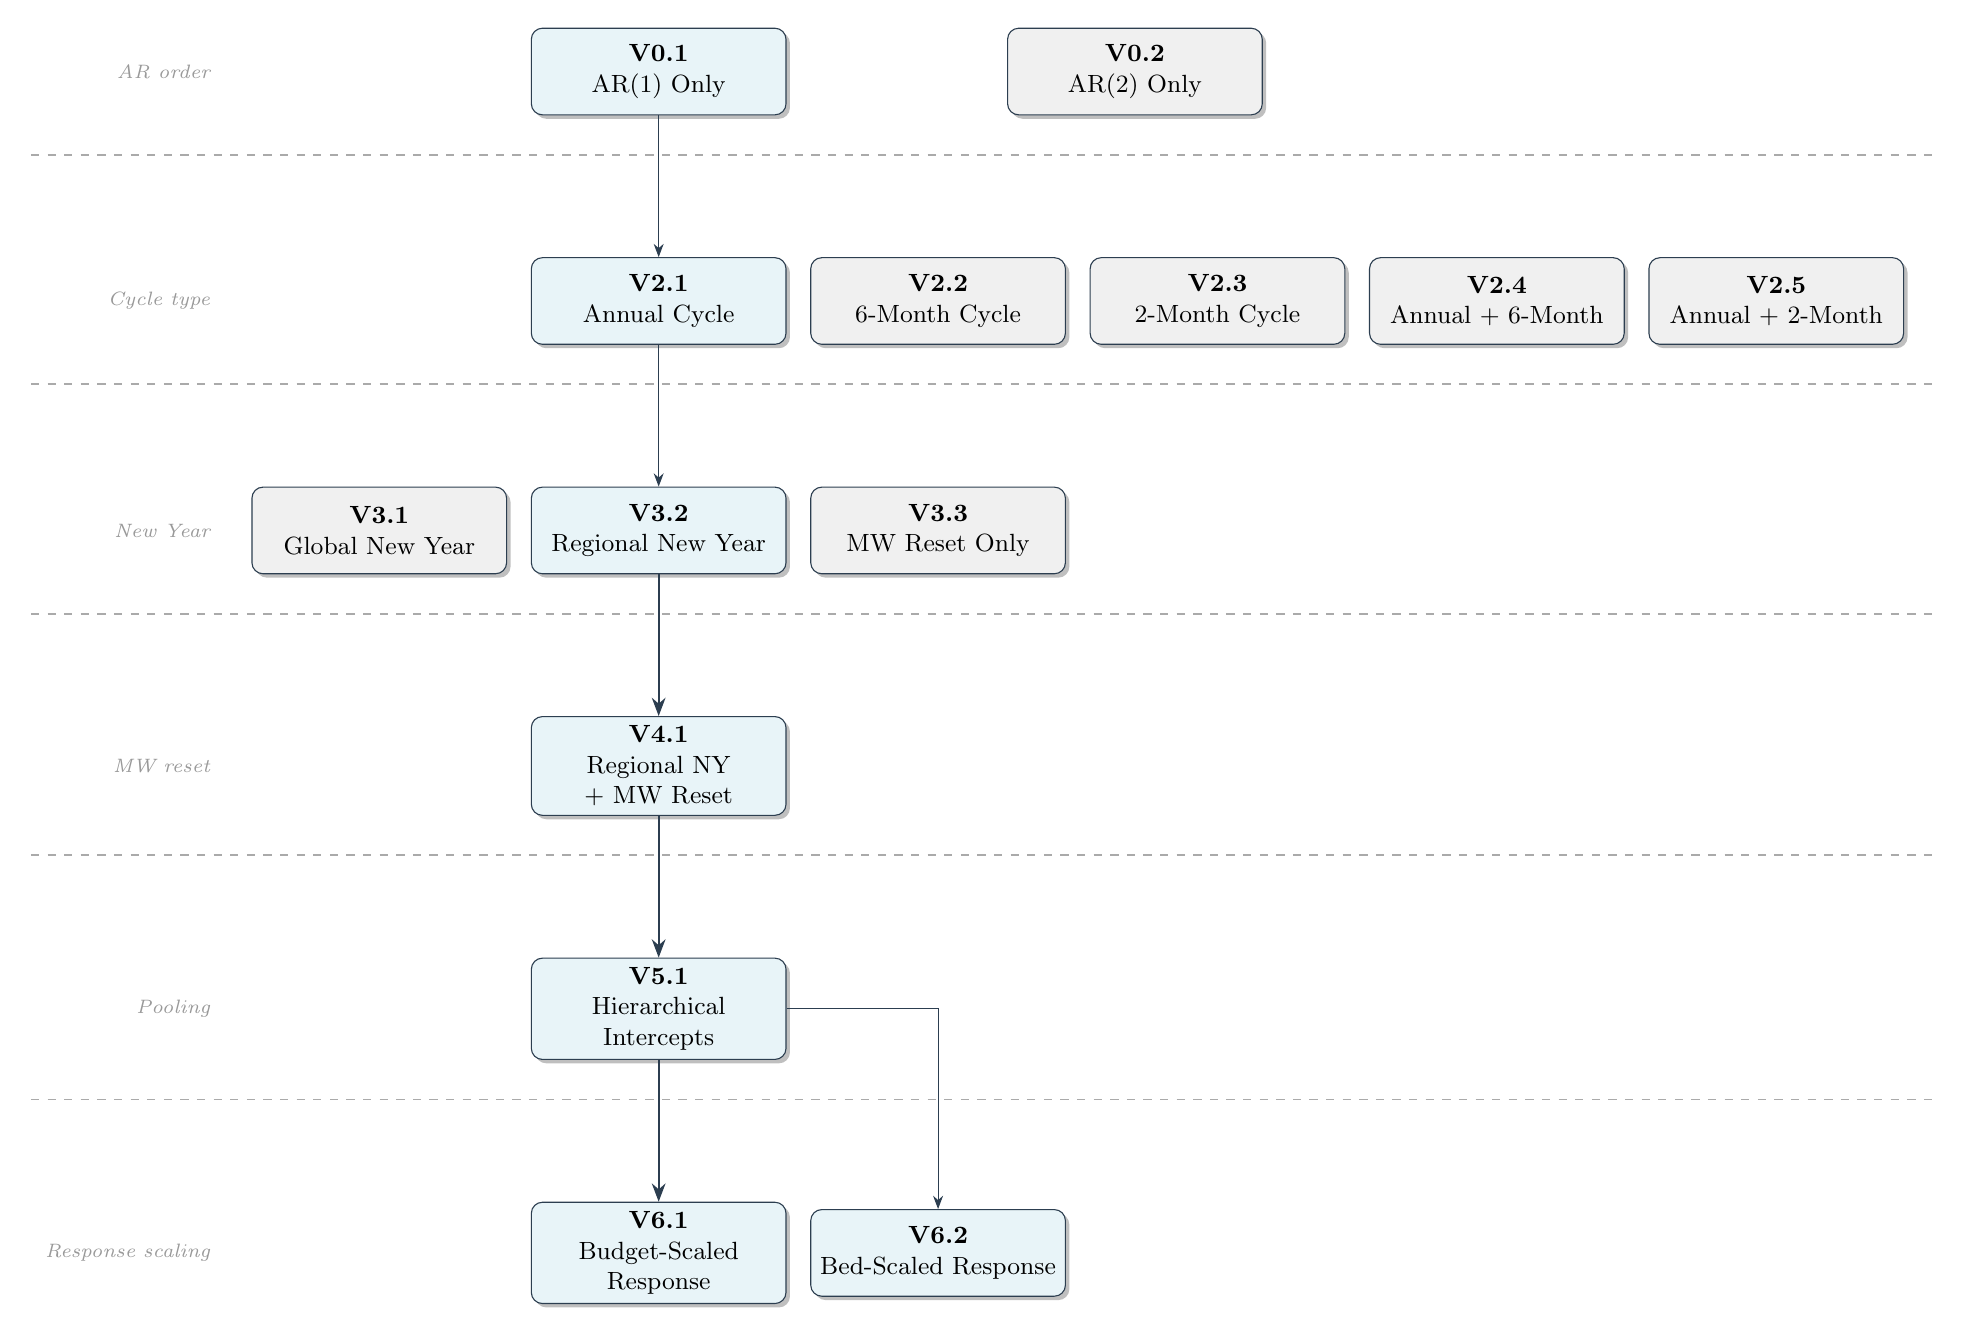
\begin{tikzpicture}[node distance=1.8cm and 0.3cm]

    % --- Row 0: AR baseline ---
    \node[model] (v0_1) {\textbf{V0.1}\\AR(1) Only};
    \node[unselected, right=2.8cm of v0_1] (v0_2) {\textbf{V0.2}\\AR(2) Only};

    % --- Row 2: Cycle tests (all on same horizontal plane) ---
    \node[model, below=of v0_1] (v2_1) {\textbf{V2.1}\\Annual Cycle};
    \node[unselected, right=of v2_1] (v2_2) {\textbf{V2.2}\\6-Month Cycle};
    \node[unselected, right=of v2_2] (v2_3) {\textbf{V2.3}\\2-Month Cycle};
    \node[unselected, right=of v2_3] (v2_4) {\textbf{V2.4}\\Annual + 6-Month};
    \node[unselected, right=of v2_4] (v2_5) {\textbf{V2.5}\\Annual + 2-Month};

    % --- Row 3: New Year effects (V3.2 is spine, directly below V2.1) ---
    \node[model, below=of v2_1] (v3_2) {\textbf{V3.2}\\Regional New Year};
    \node[unselected, left=of v3_2] (v3_1) {\textbf{V3.1}\\Global New Year};
    \node[unselected, right=of v3_2] (v3_3) {\textbf{V3.3}\\MW Reset Only};

    % --- Spine ---
    \node[model, below=of v3_2] (v4_1) {\textbf{V4.1}\\Regional NY + MW Reset};
    \node[model, below=of v4_1] (v5_1) {\textbf{V5.1}\\Hierarchical Intercepts};
    \node[model, below=of v5_1] (v6_1) {\textbf{V6.1}\\Budget-Scaled Response};
    \node[model, right=of v6_1] (v6_2) {\textbf{V6.2}\\Bed-Scaled Response};

    % --- Row side labels (all anchored at left edge of V3.1) ---
    \coordinate (llabel) at ($(v3_1.west) + (-0.4, 0)$);
    \node[row label, anchor=east] at (llabel |- v0_1)  {AR order};
    \node[row label, anchor=east] at (llabel |- v2_1)  {Cycle type};
    \node[row label, anchor=east] at (llabel |- v3_2)  {New Year};
    \node[row label, anchor=east] at (llabel |- v4_1)  {MW reset};
    \node[row label, anchor=east] at (llabel |- v5_1)  {Pooling};
    \node[row label, anchor=east] at (llabel |- v6_1)  {Response scaling};

    % --- Horizontal dividers ---
    \coordinate (left)  at ($(v3_1.west) + (-2.8, 0)$);
    \coordinate (right) at ($(v2_5.east)  + ( 0.4, 0)$);

    \draw[dashed, color=divider, line width=0.6pt]
        ($(left |- v0_1.south) + (0,-0.5)$) -- ($(right |- v0_1.south) + (0,-0.5)$);
    \draw[dashed, color=divider, line width=0.6pt]
        ($(left |- v2_1.south) + (0,-0.5)$) -- ($(right |- v2_1.south) + (0,-0.5)$);
    \draw[dashed, color=divider, line width=0.6pt]
        ($(left |- v3_2.south) + (0,-0.5)$) -- ($(right |- v3_2.south) + (0,-0.5)$);
    \draw[dashed, color=divider, line width=0.6pt]
        ($(left |- v4_1.south) + (0,-0.5)$) -- ($(right |- v4_1.south) + (0,-0.5)$);
    \draw[dashed, color=divider, line width=0.6pt]
        ($(left |- v5_1.south) + (0,-0.5)$) -- ($(right |- v5_1.south) + (0,-0.5)$);

    % --- Arrows ---
    \draw[arr branch] (v0_1) -- (v2_1);
    \draw[arr branch] (v2_1) -- (v3_2);
    \draw[arr] (v3_2) -- (v4_1);
    \draw[arr] (v4_1) -- (v5_1);
    \draw[arr] (v5_1) -- (v6_1);
    \draw[arr branch] (v5_1) -| (v6_2);

\end{tikzpicture}
\end{document}
